%!TEX root = ../thesis_phd.tex
%%%%%%%%%%%%%%%%%%%%%%%%%%%%%%%%%%%%%%%%%%%%%%%%%%%%%%%%%%%%%%%%%%%%%%%%%%%%%%%%
% oscillation_analysis.tex: Analysis of Neutrino Oscillations:
%%%%%%%%%%%%%%%%%%%%%%%%%%%%%%%%%%%%%%%%%%%%%%%%%%%%%%%%%%%%%%%%%%%%%%%%%%%%%%%%
\chapter{Analysis}
\label{analysis_chapter}
%%%%%%%%%%%%%%%%%%%%%%%%%%%%%%%%%%%%%%%%%%%%%%%%%%%%%%%%%%%%%%%%%%%%%%%%%%%%%%%%

A measurement of parameters \deltamtht and \thetatth is obtained from
a likelihood fit to the FD data, namely the reconstructed energy spectrum.
Performing such a fit requires a prediction of the FD spectrum which can be
varied in terms of the oscillation parameters.
A naive approach would be to generate a FD prediction straight from
FD Monte Carlo (MC) simulation.
That approach, however, would be quite sensitive to systematic errors,
in particular due to uncertainties  in the \numi flux and neutrino
cross sections.
\nova's two-detector design is aimed precisely at mitigating the effects of
such uncertainties; the ND can be used to determine the expected
spectrum at the FD in a way which mostly cancels the large uncertainties the
the MC prediction.
The procedure of generating the FD prediction in terms of the observed
ND spectrum, referred to as \textit{extrapolation}, is described in Section
\ref{extrap_section}.
The fitting procedure is described in Section \ref{fitting_section}.

\begin{figure}
\begin{center}
  \begin{subfigure}[b]{0.8\textwidth}
    \centering
    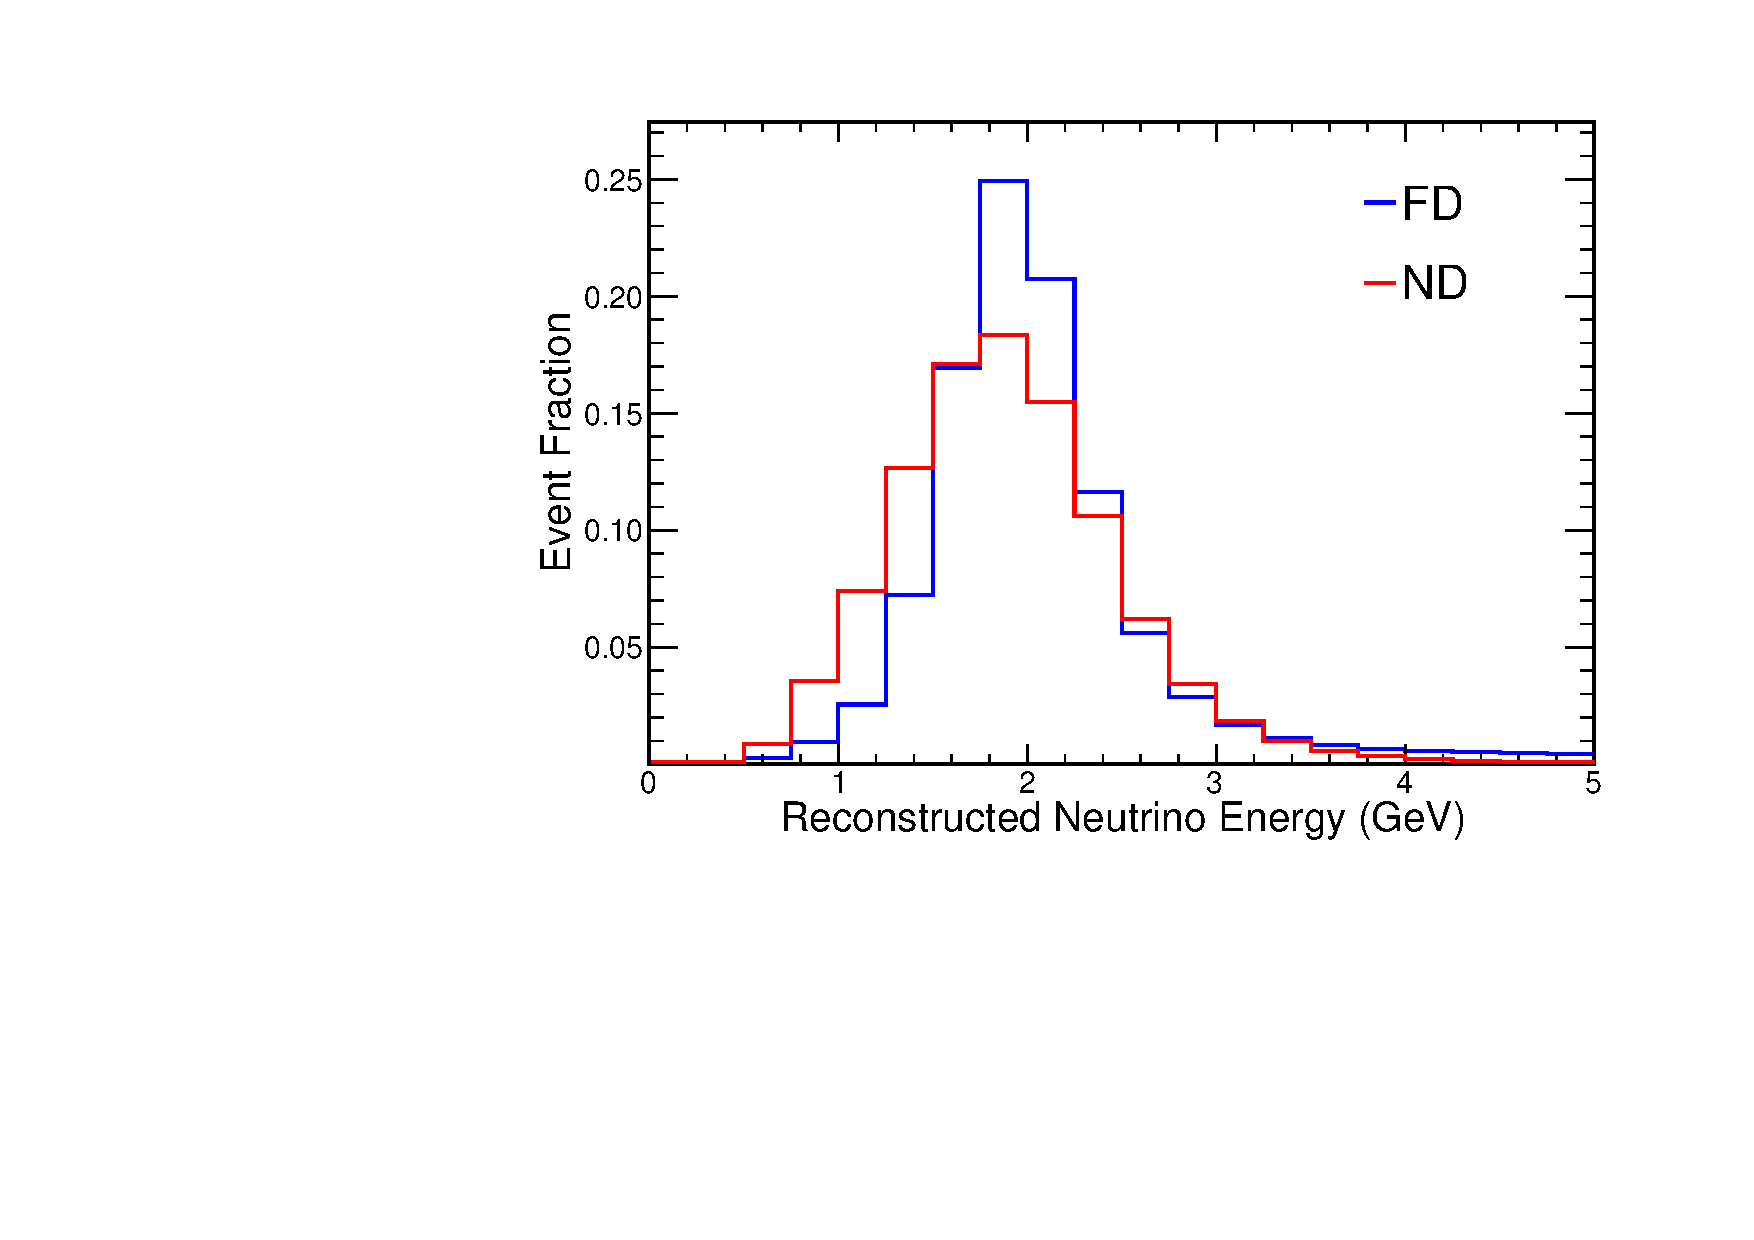
\includegraphics[width=\textwidth]{figures/plots/extrap/fd_nd_spec.pdf}
  \end{subfigure}

  \begin{subfigure}[b]{0.8\textwidth}
    \centering
    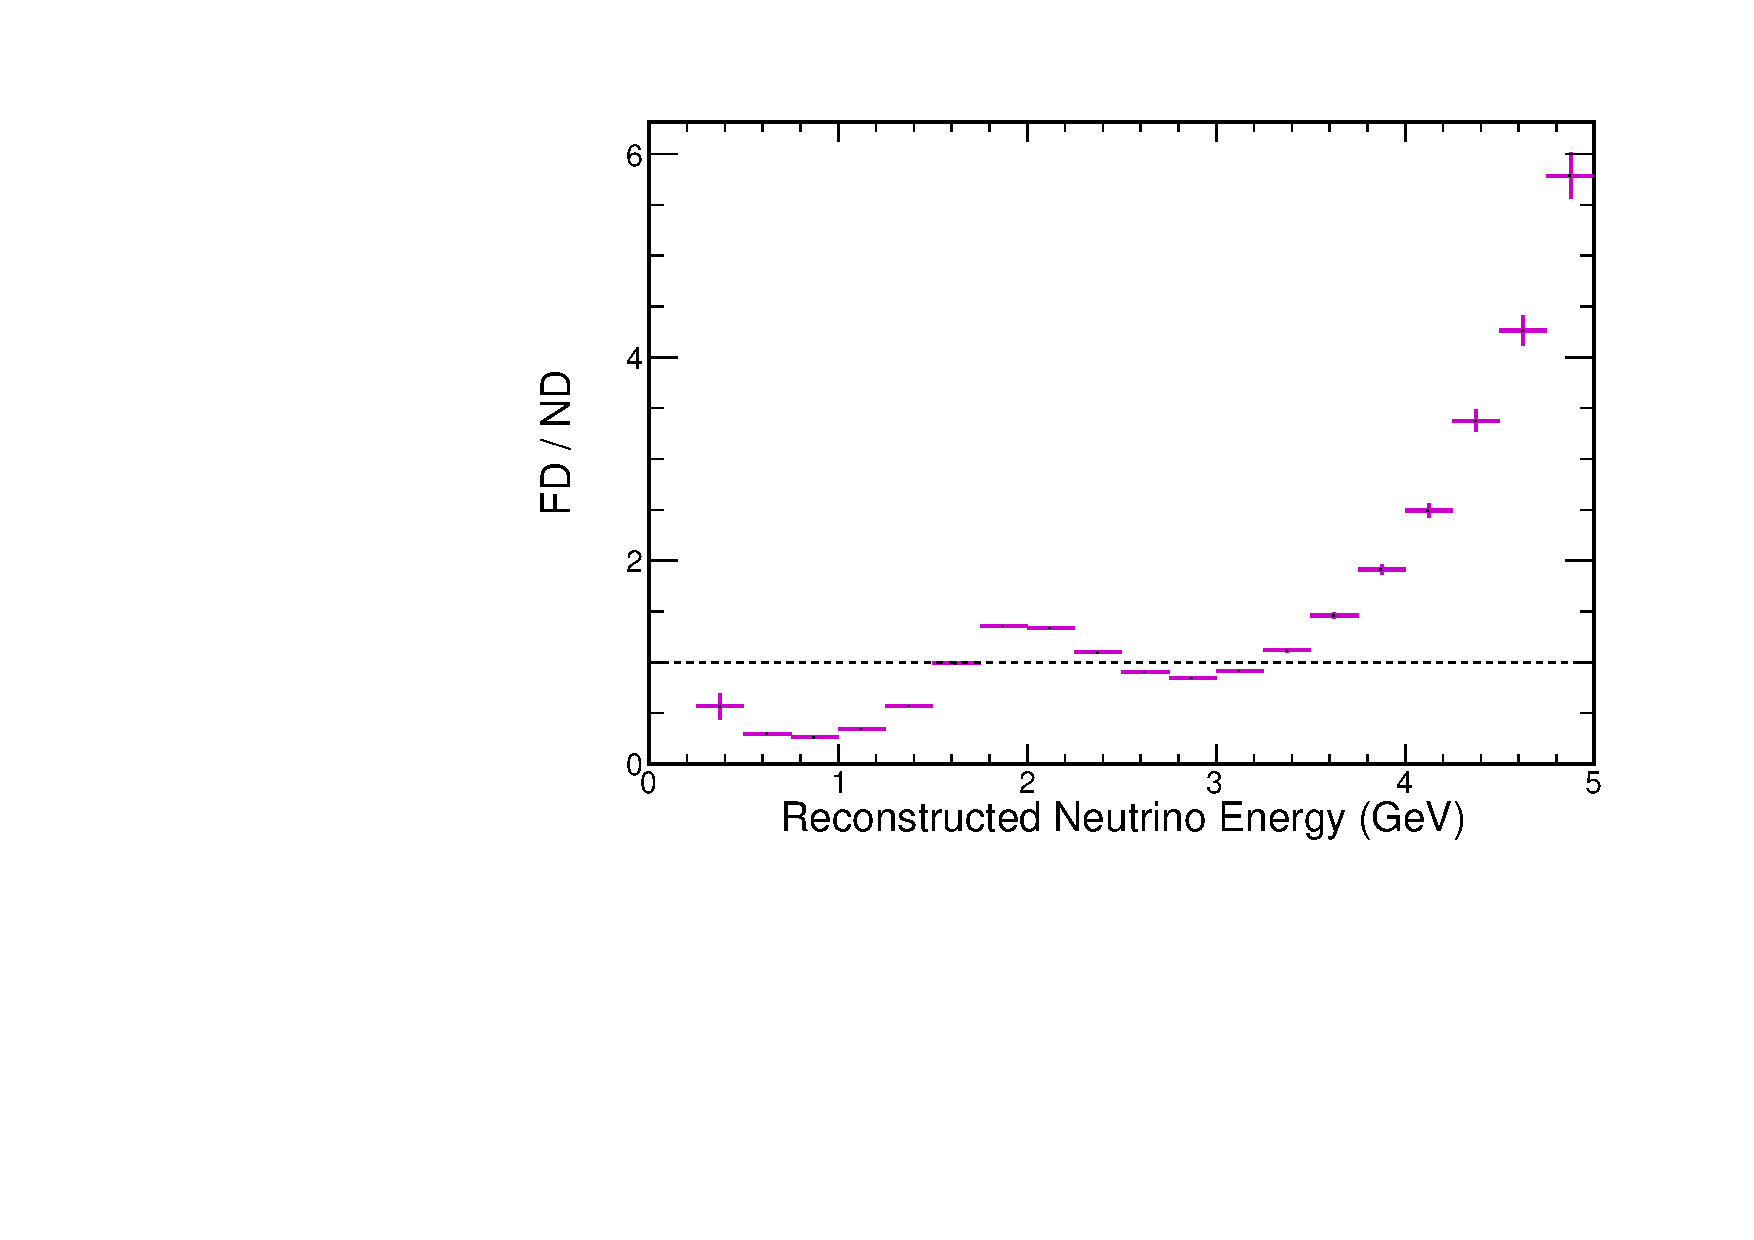
\includegraphics[width=\textwidth]{figures/plots/extrap/fd_nd_ratio.pdf}
  \end{subfigure}

\end{center}
\caption{MC Prediction for ND and FD}{
The observed ND and FD event energy specta display different characteristics
primarily due to geometric effects.
The small size of the ND a bias towards containment of lower energy events.
Also, proximity to the \numi source causes the ND to observe a wider
range of solid angle, effectively broadening the energy peak.
The top pane shows the overlaid ND and FD spectra taken from MC, with each
histogram scaled to unit area to highlight shape differences.
The bottom pane shows the ratio of the two spectra.
Note that the ratio is not used in the extrapolation procedure; instead,
the ratio of the true spectra is used to transfer from ND to FD.
}
\label{ratioNDFD}
\end{figure}

\section{Prediction and Extrapolation}
\label{extrap_section}

The FD prediction is built from signal and background components.
In total, the prediction is built up from \numu CC signal, beam-induced
background components, and cosmic-ray background.
As the dominant component, the \numu CC signal is extrapolated from
ND data to take the observed spectrum into account.
Beam backgrounds, on the other hand, are taken straight from MC simulation.
The cosmic cosmic-ray background component is taken from data recorded
in the absence of the \numi beam signal, referred to as the
\textit{out-of-time sideband}.

\subsection{\numu CC Signal Extrapolation}
\label{sig_extrap_section}
Naively, one might expect that the ratio of the FD spectrum to the ND spectrum
could be directly interpreted as an oscillation probability.
This naive approach is complicated by two factors.
First, the ND and FD spectra are independently shaped by various geometric
and other systematic effects.
Second, the imperfect resolution of the energy estimator causes
distortion of the measured spectra which is inconsistent across detectors.
The extrapolation procedure aims to mitigate both of these factors.

Geometric effects form the majority of the discrepancy between the
ND and FD spectra.
Foremost, the ND is a small detector.
The energy spectrum observed by ND is thus shaped by the topologies
of events which can be contained within the detector.
As a result, the ND spectrum is biased towards events with
smaller hadronic showers and shorter muon tracks, although the steel planes
of the muon catcher helps to mitigate the latter problem.
Additionally, even though the ND is considerably smaller than the FD,
it subtends a much larger solid angle relative to the \numi source.
As a result, it sees pions decaying over a wider range of off-axis angle
and thus a broader energy spectrum than the FD.


The geometric effects which shape the ND and FD spectra is well modeled
by the MC simulation.
Selection effects induced by the detector size are handled by simulating
with an accurately sized detector.
The beam acceptance issue is covered well by the beam simulation described in
Section \ref{beam_sim_section}; uncertainties in the beam situation are
treated as a systematic error.
The discrepancy between the FD and ND spectra is shown in Figure
\ref{ratioNDFD}.


The extrapolation procedure also aims to capture the smearing effect of
imperfect energy energy resolution independently in each detector.
This is accomplished by forming a 2D histogram of reconstructed energy
vs. true energy in each detector, referred to as the \textit{reco-true matrix}.
These histograms can be used to reweight between the reconstructed
and true spectra in either detector.

Ultimately, extrapolation from ND to FD is performed in bins of true energy.
First, the ND data spectrum is reweighted (bin-by-bin)
using the ND reco-true matrix
to reproduce the observed ND spectrum in bins of true energy.
Each bin in that spectrum is then reweighted in terms of FD/ND true energy
ratios to
produce an FD prediction in bins of true energy.
Oscillation probabilities are applied to the FD true bins.
The bins in the
oscillated true prediction are then reweighted in using the FD reco-true
matrix to produce the final FD prediction in bins of true energy.
A schematic view of the extrapolation procedure can be seen in Figure
\ref{extrap_fig}.

\begin{figure}
\begin{center}
  \begin{subfigure}[b]{\textwidth}
    \centering
    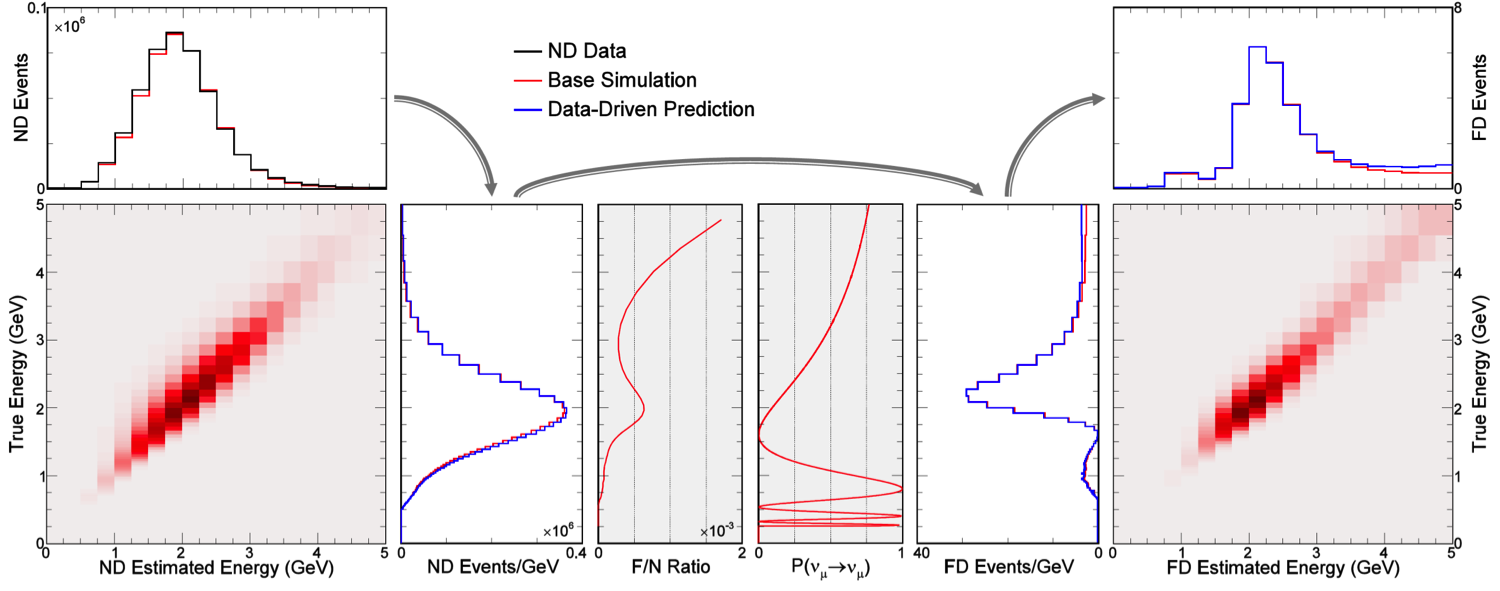
\includegraphics[height=0.45\textwidth, angle=-90]{figures/figures/extrap_schematic.png}
  \end{subfigure}
\end{center}
\caption{Schematic view of the extrapolation}{
Extrapolation of \numu CC signal is performed in bin-by-bin.
The reconstructed ND energy spectrum is first reweighted to true energy
using the ND reco-true matrix.
Reweighted ND true energy is then transferred to the FD spectrum using the
F/N ratio.
Oscillation probabilities are applied to true energy bins,
then a prediction in reconstructed energy is produced using the
FD true-reco matrix.
Selected event spectra shown here do not correspond to those
involved in this analysis, graphic only serves as a schematic overview.
}
\label{extrap_fig}
\end{figure}

\subsection{Background Prediction}

Only the \numu and $\bar{\nu}_\mu$ components are given the full extrapolation
treatment.
The beam-induced background components -- NC, \nue, $\bar{\nu}_e$, \nutau and
$\bar{\nu}_\tau$ -- are all taken directly from the MC prediction.
Since these components are small, taking these components does not incur
a significant error.
In practice, this means that the ND MC prediction for each background component
is subtracted from the ND data prior to extrapolation.
Once the extrapolated FD prediction has been generated, each predicted MC
background component is added.


Cosmic-ray background is estimated using selected events from the out-of-time
sideband in FD data.
While each \numi beam spill spans only 10 $\mu$s, the functional readout window
spans 450 $\mu$s.
The excess data which surrounds the beam spill forms the out-of-time sideband.
Sideband data is convenient for this purpose because it trivially
matches the exposure of the in-time data using a simple factor $f$:
\begin{equation}
f = \frac{10~\mu\text{s}}{ 450~\mu\text{s} - 10~\mu\text{s}} = \frac{1}{44}
\end{equation}
Similar to the FD beam-induced background prediction, the cosmic-ray
background prediction is added directly to the extrapolated FD signal
prediction.


\begin{figure}
\begin{center}
  \begin{subfigure}[b]{0.8\textwidth}
    \centering
    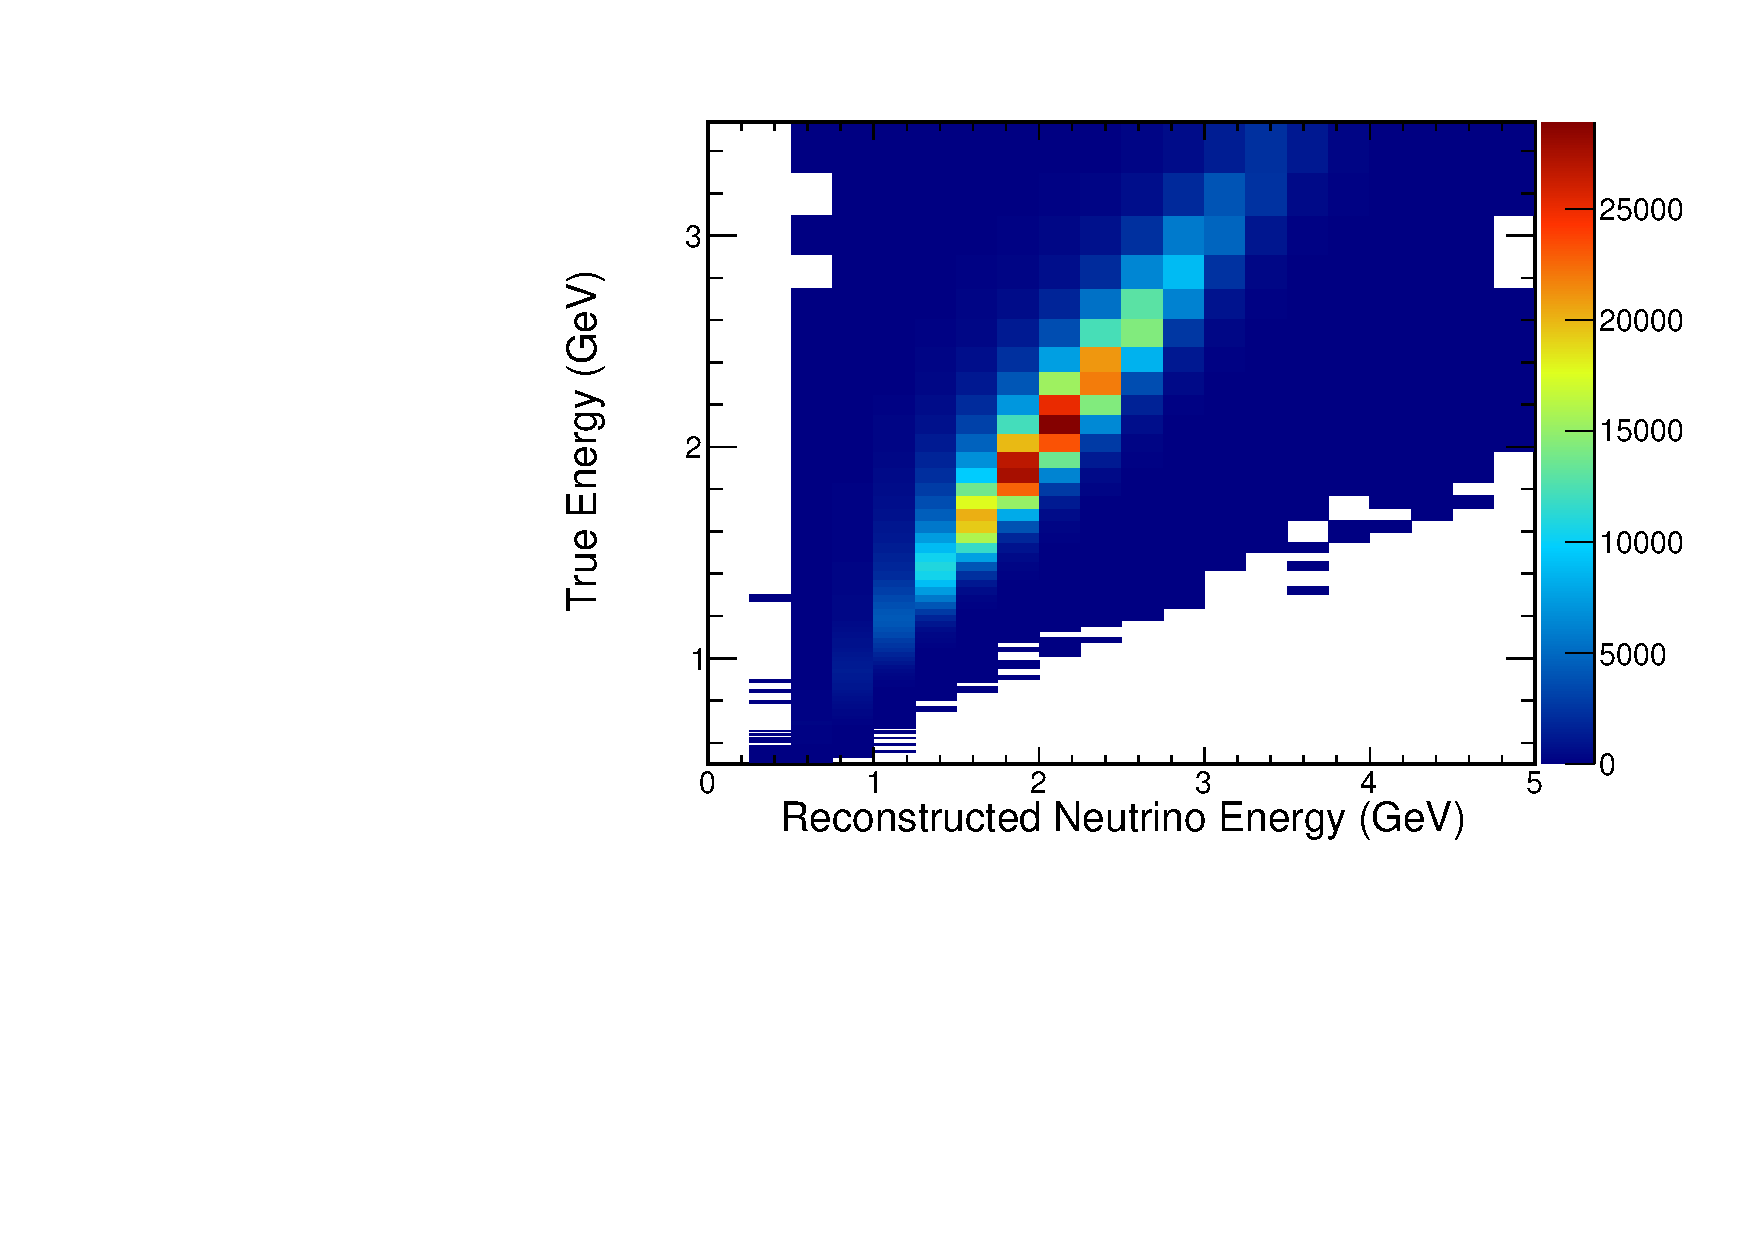
\includegraphics[width=\textwidth]{figures/plots/extrap/NDRecoToTrue.pdf}
  \end{subfigure}

  \begin{subfigure}[b]{0.8\textwidth}
    \centering
    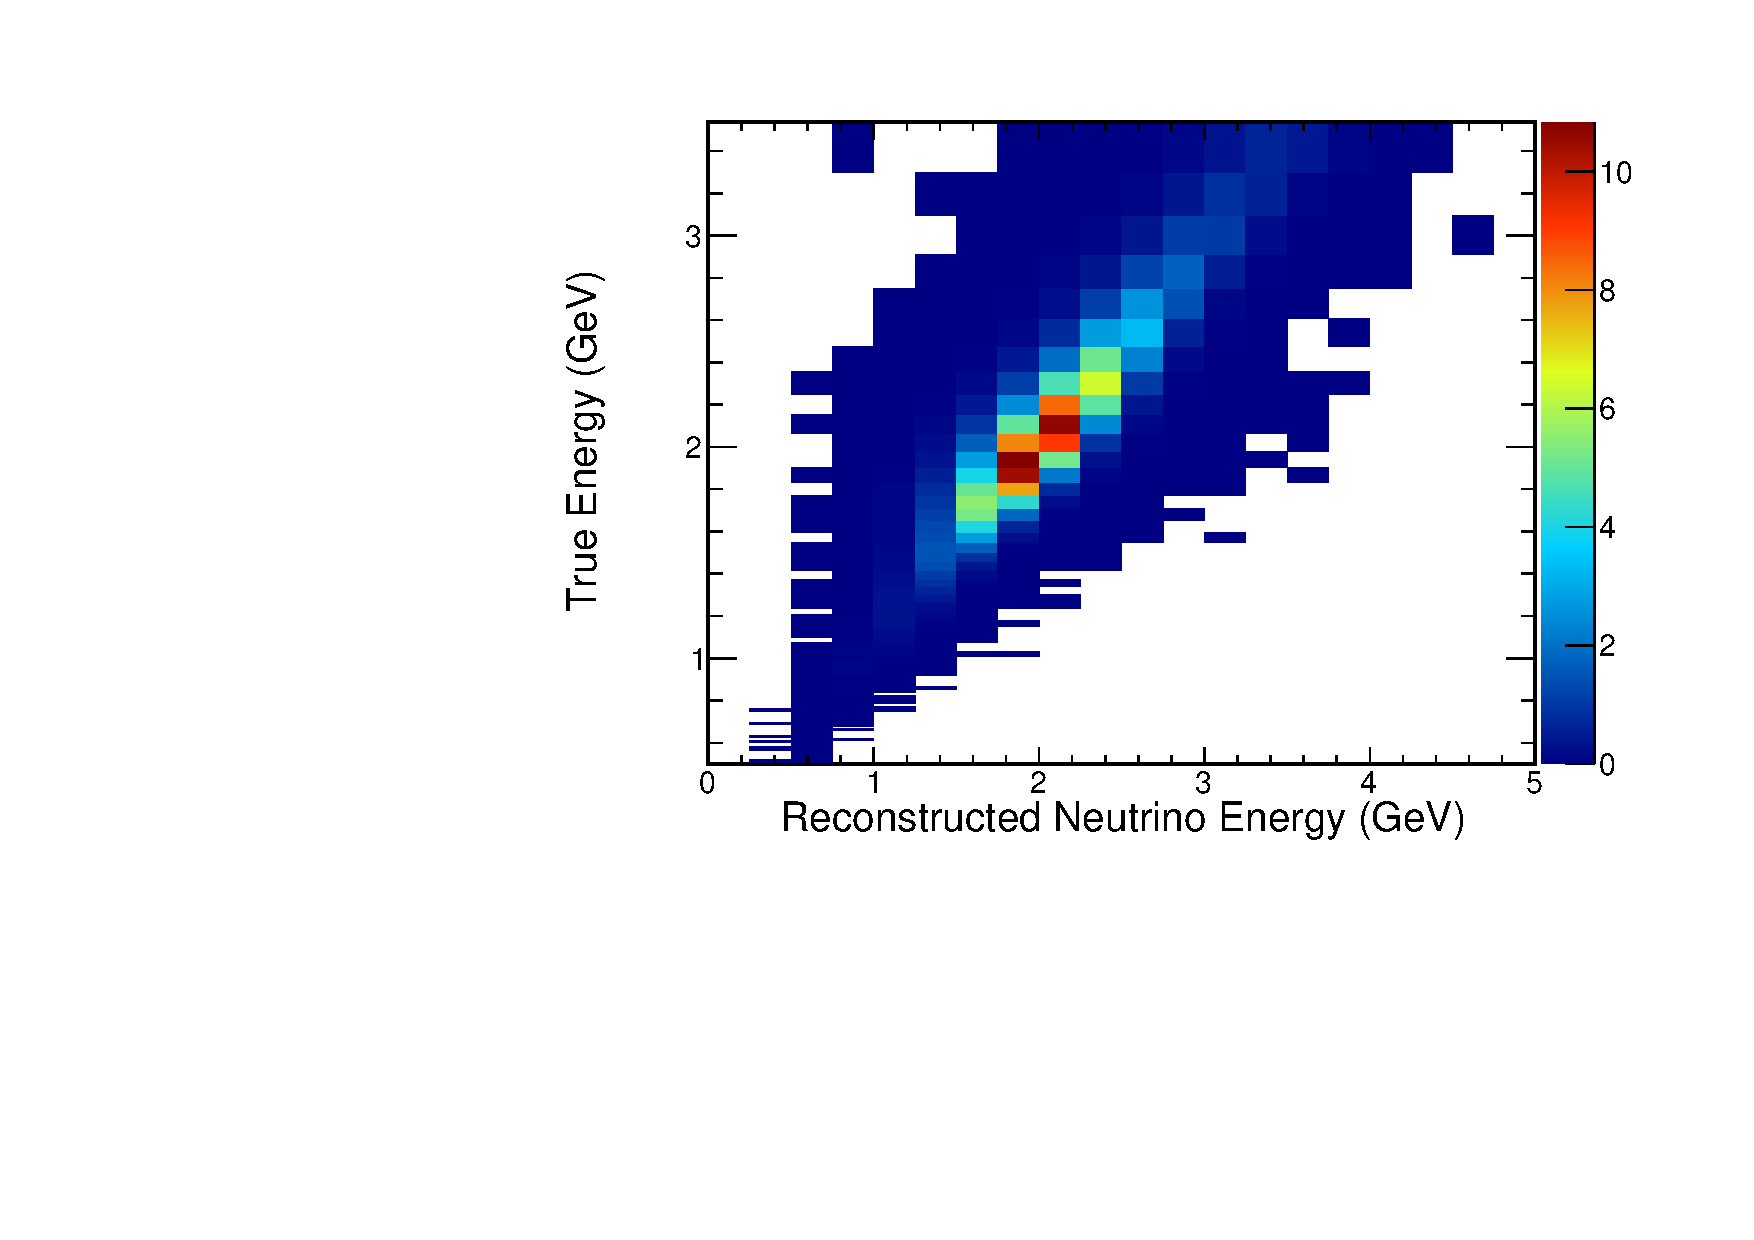
\includegraphics[width=\textwidth]{figures/plots/extrap/FDTrueToReco.pdf}
  \end{subfigure}

\end{center}
\caption{ND and FD reco-true reco-true matrices}{
The ND and FD reco-true matrices are used to spectra between
reconstructed and true energy.
The ND reco-true matrix, top, is used to convert the ND data reconstructed
energy spectrum to a reweighted true energy representation.
The FD reco-true spectrum is used to convert a predicted FD extrapolated
true energy spectrum to a reconstructed energy spectrum.
}
\label{extrapRecoTrue}
\end{figure}



\begin{figure}
\begin{center}
  \begin{subfigure}[b]{0.8\textwidth}
    \centering
    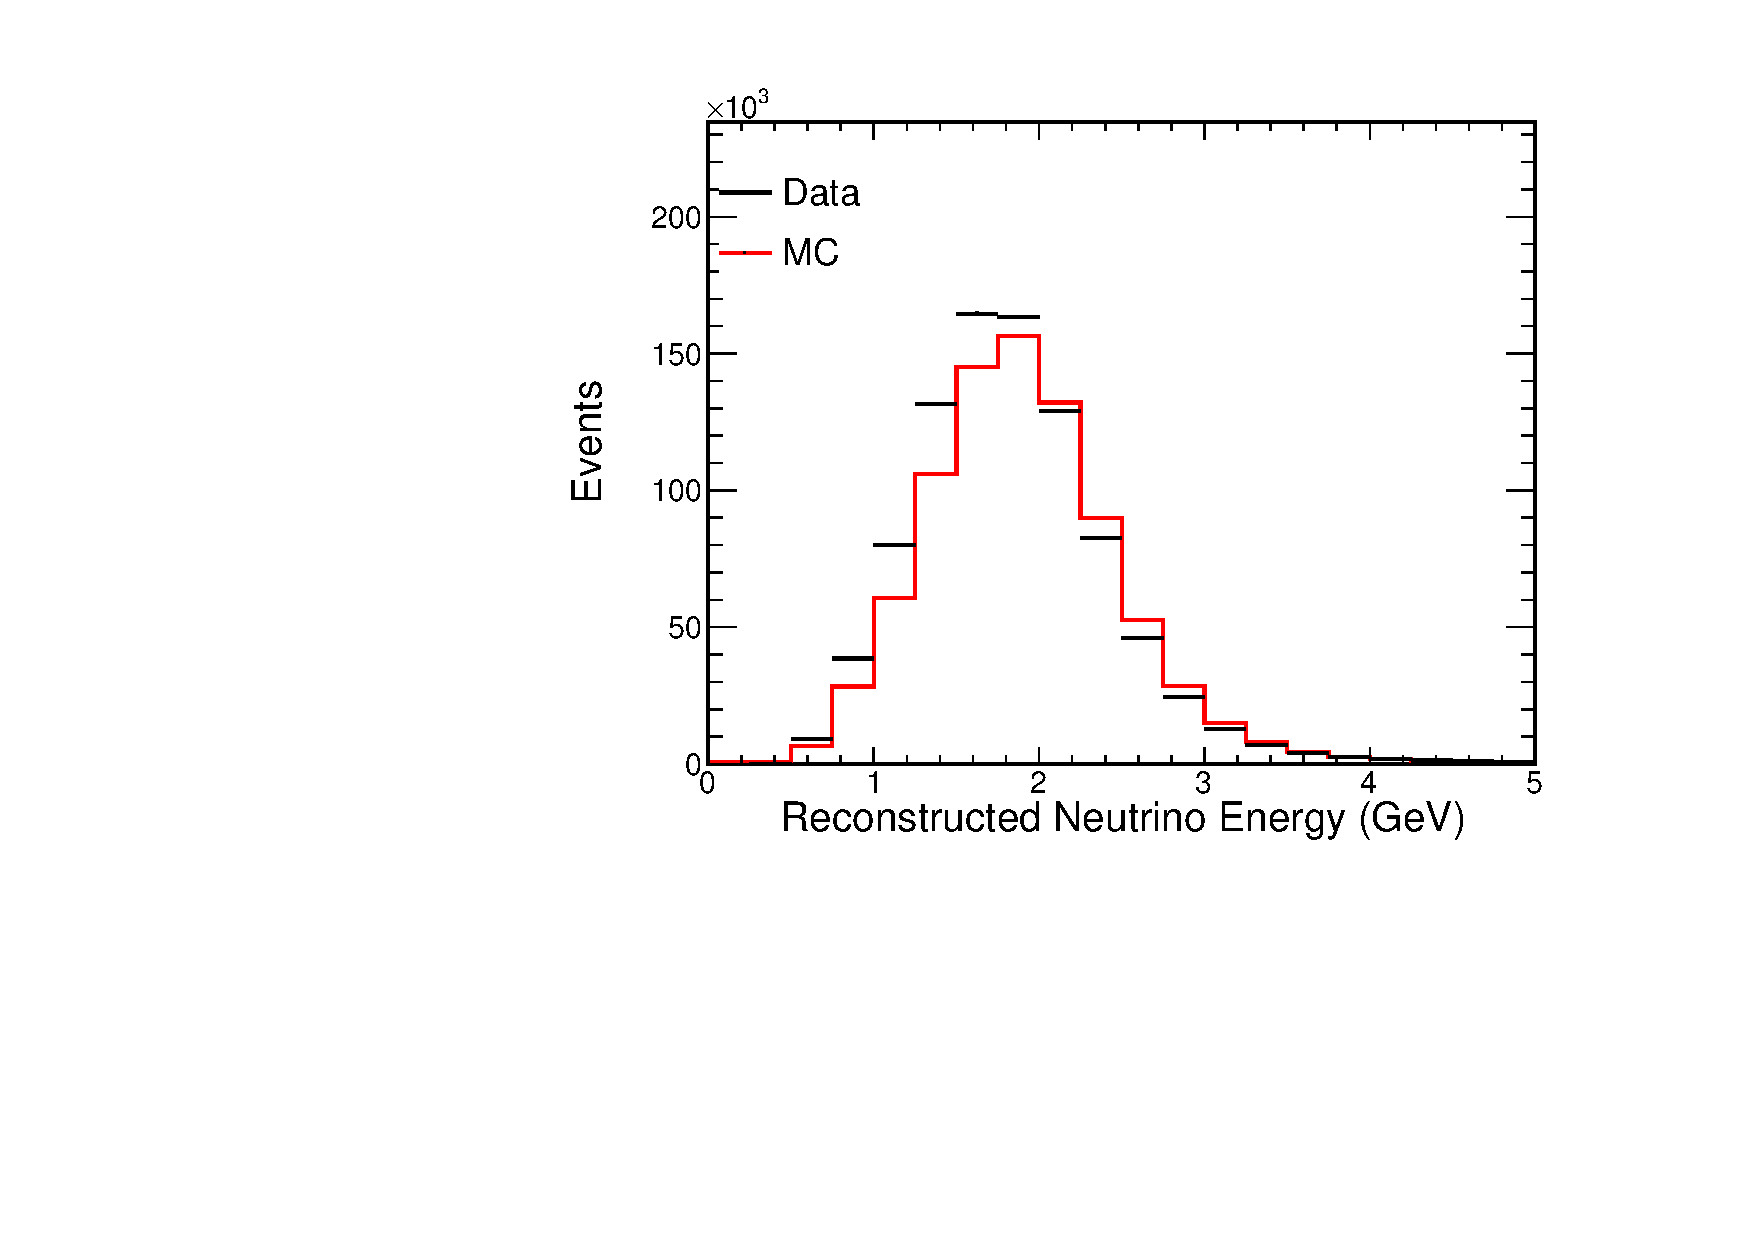
\includegraphics[width=\textwidth]{figures/plots/extrap/NDReco.pdf}
  \end{subfigure}

  \begin{subfigure}[b]{0.8\textwidth}
    \centering
    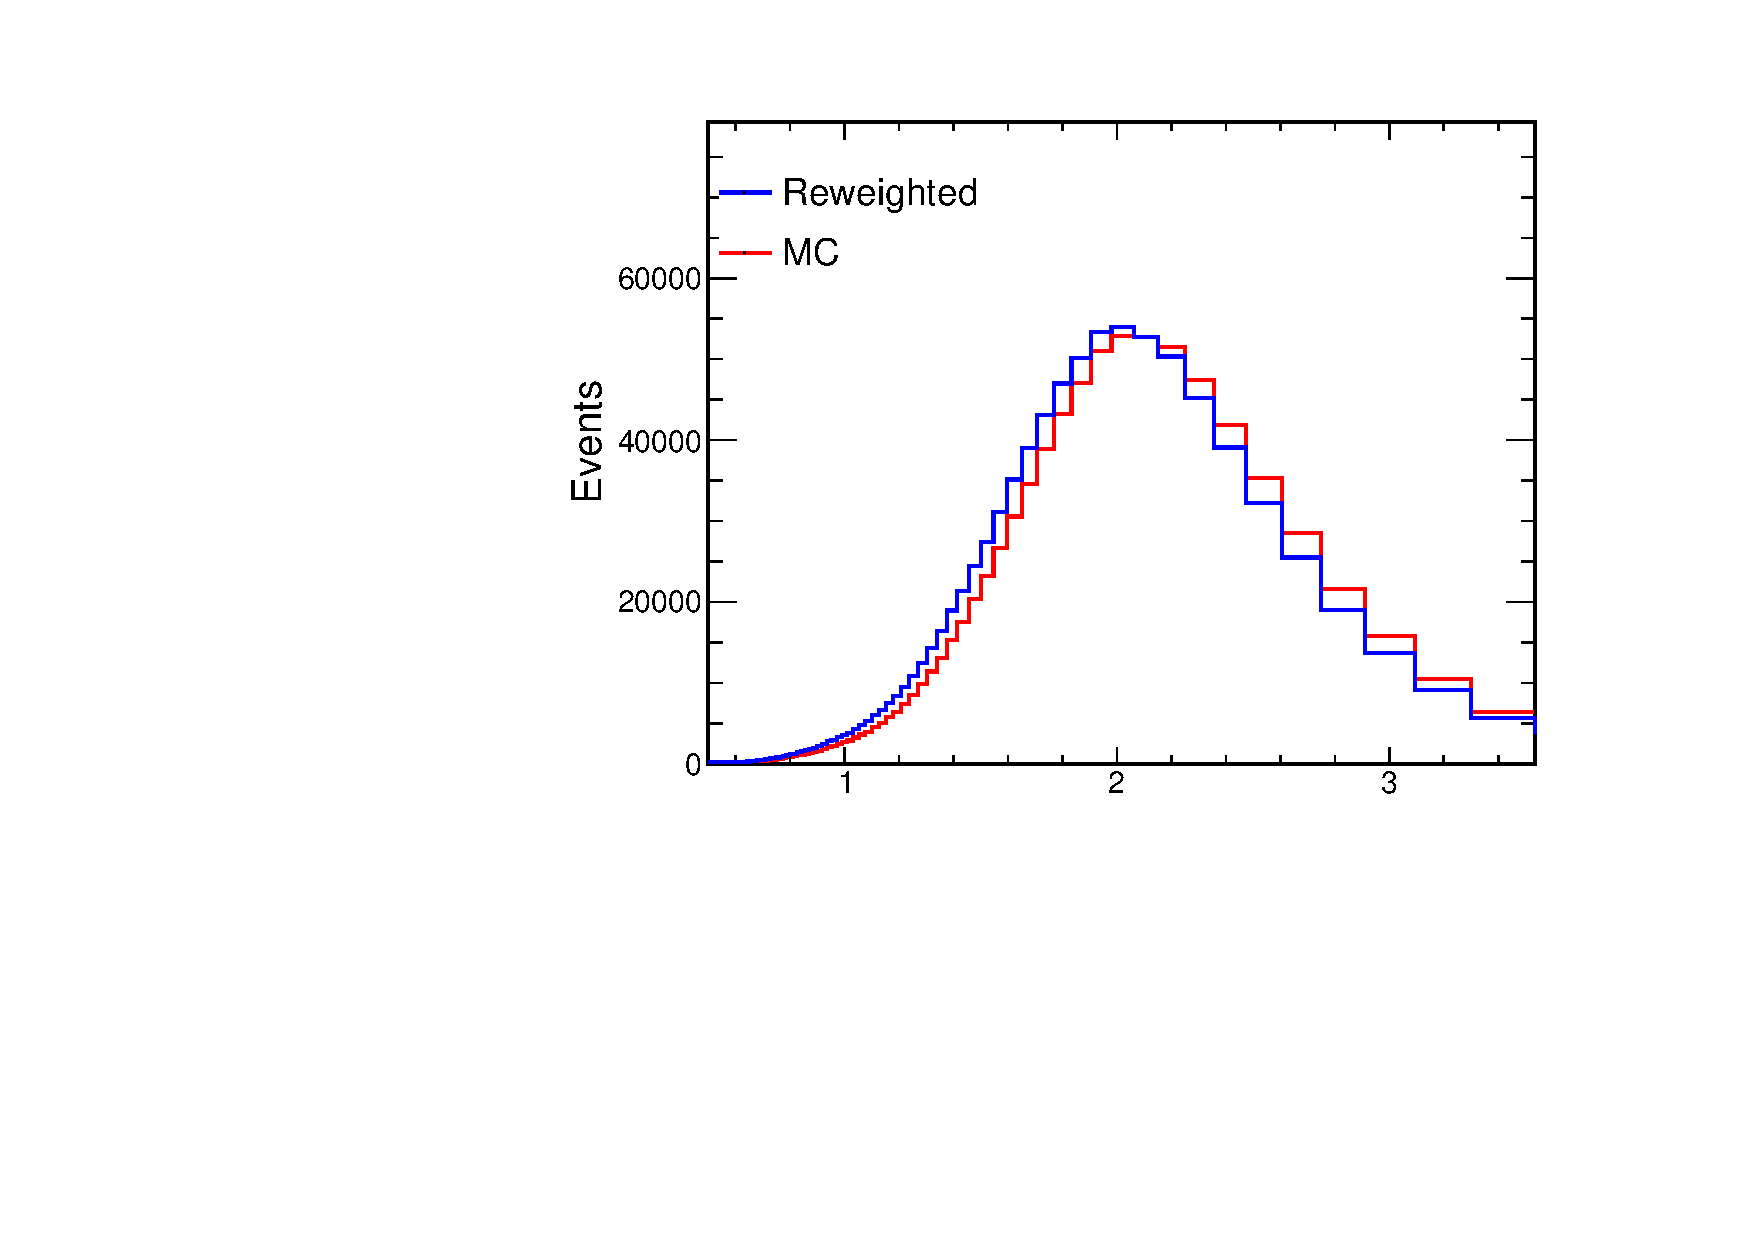
\includegraphics[width=\textwidth]{figures/plots/extrap/NDTrue.pdf}
  \end{subfigure}

\end{center}
\caption{ND spectra: reconstructed, data, true and reweighted}{
The reconstructed energy spectrum in ND data (top, black) is used to adjust the
MC prediction (bottom and top, red).
The MC prediction is reweighted bin-by-bin based on the reco-true matrix
(Figure \ref{extrapRecoTrue}) to produce the reweighted prediction, blue.
}
\label{extrapNDDataRecoTrue}
\end{figure}

\begin{figure}
\begin{center}
  \begin{subfigure}[b]{0.8\textwidth}
    \centering
    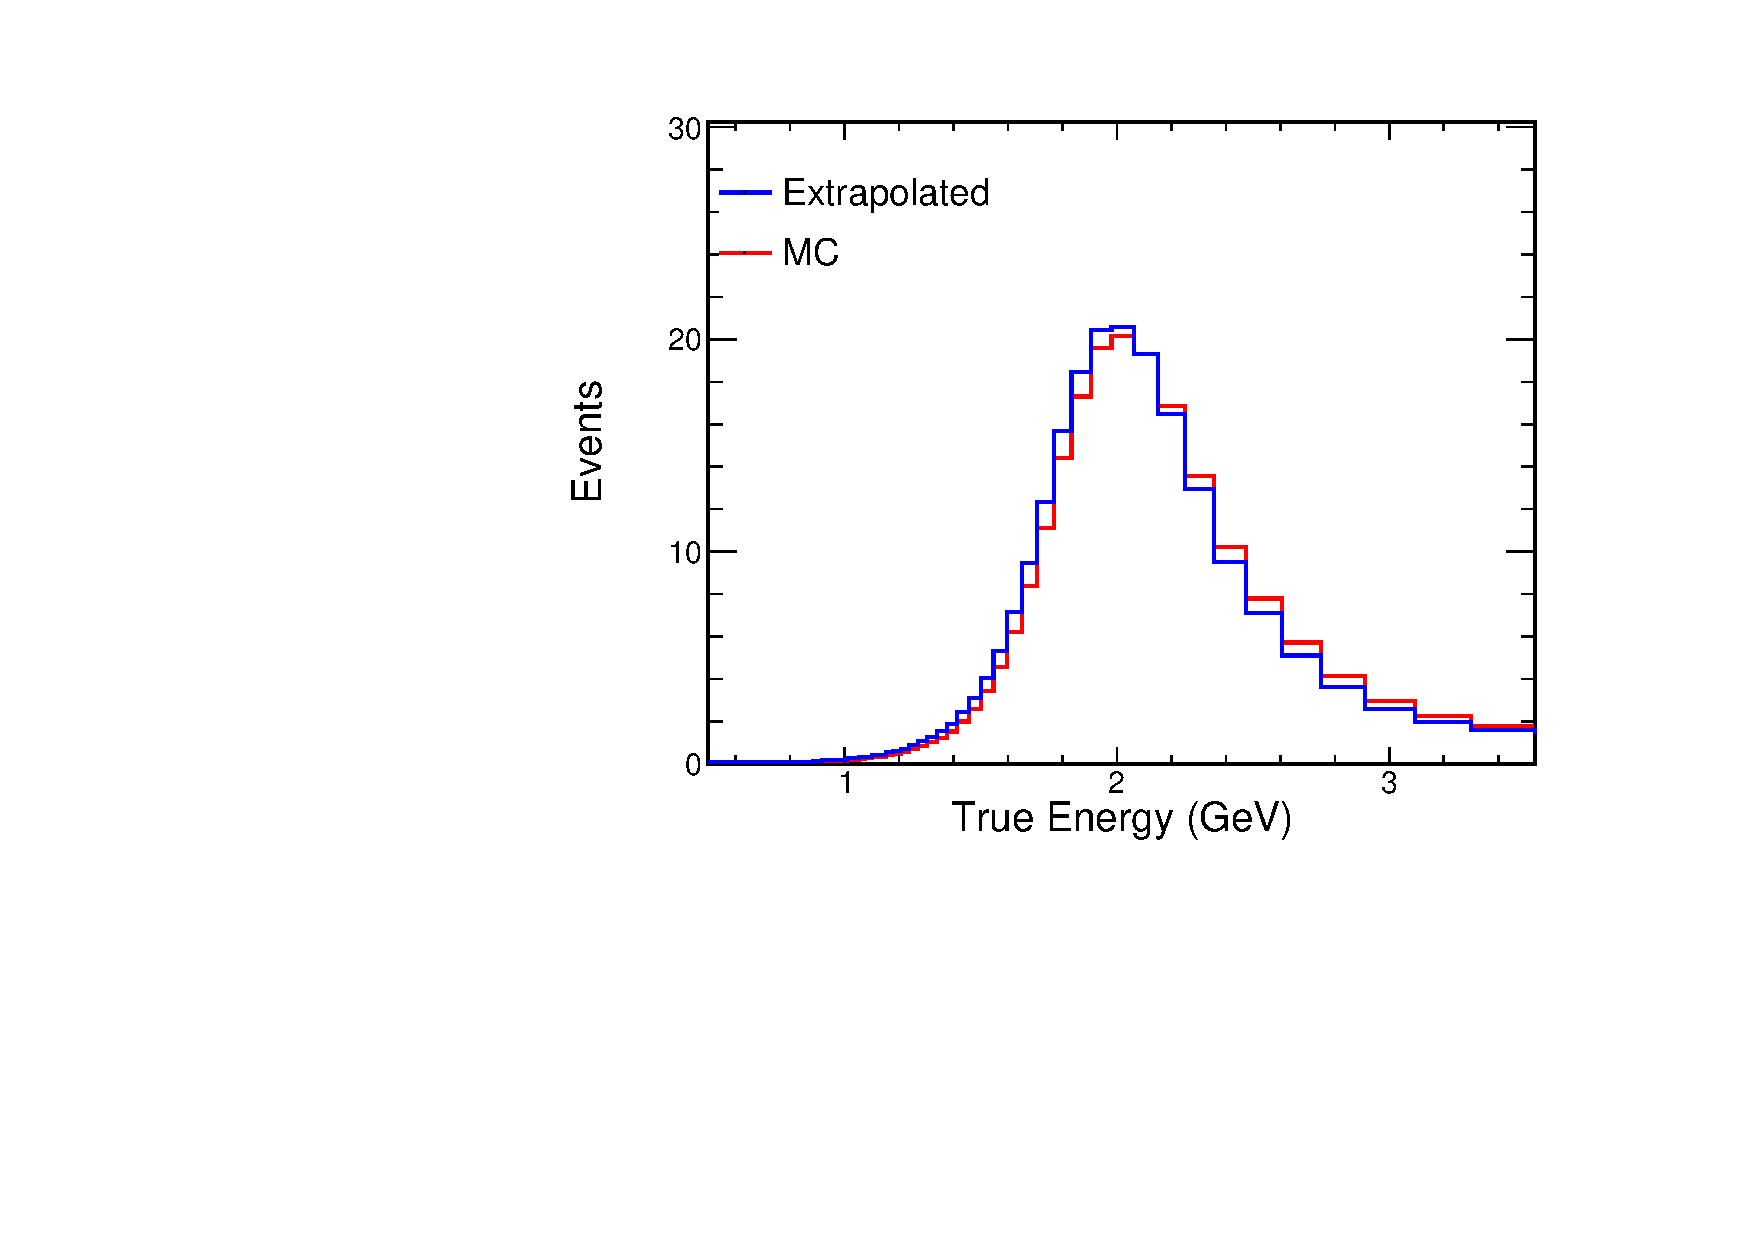
\includegraphics[width=\textwidth]{figures/plots/extrap/FDTrue.pdf}
  \end{subfigure}

  \begin{subfigure}[b]{0.8\textwidth}
    \centering
    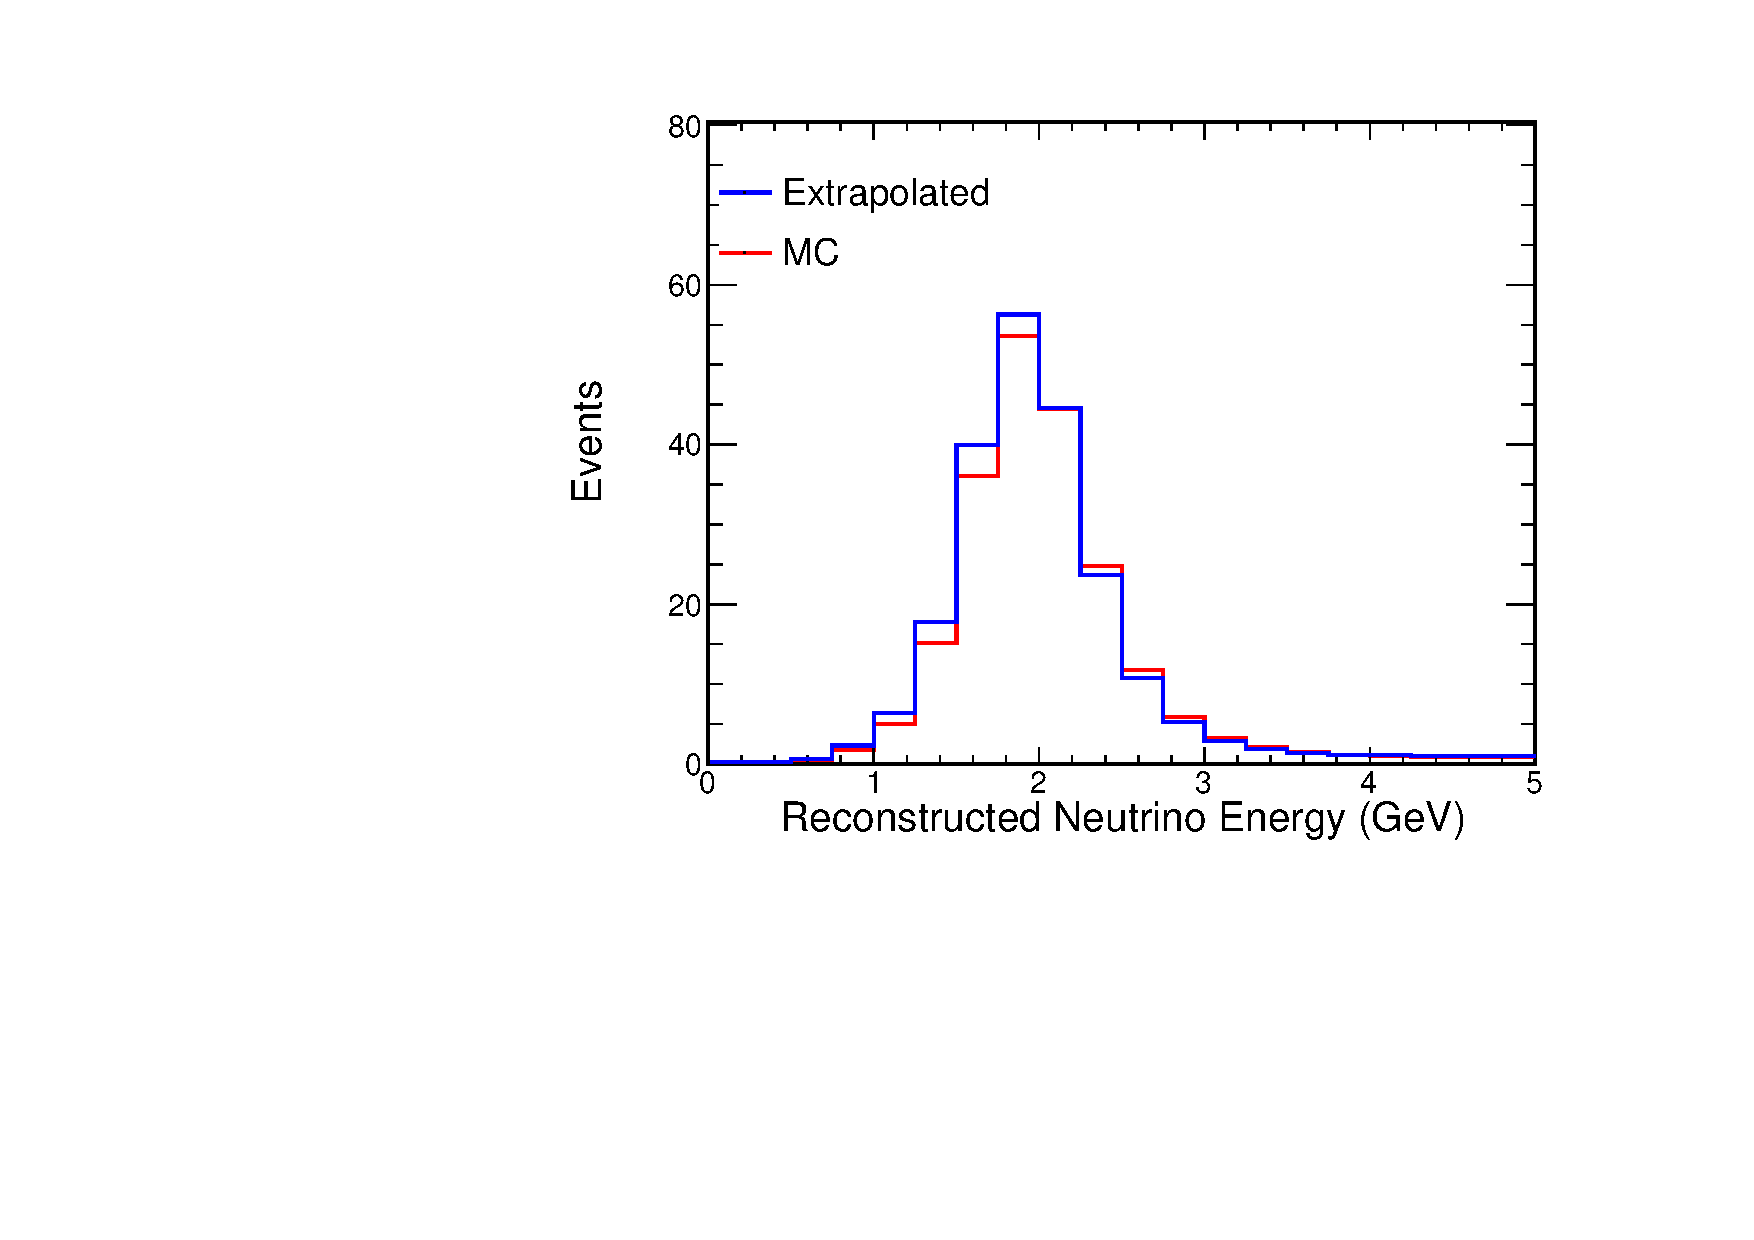
\includegraphics[width=\textwidth]{figures/plots/extrap/FDReco.pdf}
  \end{subfigure}


\end{center}
\caption{FD prediction: reconstructed, true and reweighted}{
The red spectra in both the top and bottom pane show the straight FD MC
prediction in bins of true and  reconstructed energy, respectively.
In the top pane, the blue spectrum is constructed by applying
the FD/ND ratio to the ND true energy spectrum shown in Figure
\ref{extrapNDDataRecoTrue}.
The corresponding blue spectrum in the bottom pane has been reweighted
based on the reco-true matrix in Figure \ref{extrapRecoTrue} to produce the
final FD prediction.
In this case, no oscillation probabilities have been applied to the true bins,
thus showing the predicted spectrum for the case that neutrino oscillation
did not occur.
}
\label{extrapFDRecoTrue}
\end{figure}

\subsection{Detector Configurations}

The \nova FD installation procedure and Data Acquisition (DAQ) system were
designed with an ability to provide readout of a partial detector.
It is not uncommon for the detector to operate in a configuration where
one or more \textit{blocks} (as described in section \ref{cell_section}),
of the detector are left out of the readout.
Much of the data used in this analysis was recorded while the \nova FD
was still under construction, meaning that absent blocks are common
in the data.

An accurate FD prediction thus relies on an accurate representation
of the detector configurations in the MC simulation.
This is achieved enumerating the detector configurations
used in the data and aggregating the exposure (POT) recorded
in each configuration.
The FD MC sample is then constructed by proportionally allocating
the appropriate exposure to each detector configuration.

\section{Fitting}

\label{fitting_section}

\subsection{Maximum-likelihood Fitting}
\label{bayesian_fitting_section}

A binned maximum-likelihood procedure is used to measure oscillation parameters
\deltamtht and \thetatth by comparing the extrapolated FD prediction to the
observed FD data.
The prediction is cast as a function of the oscillation parameters
through by applying oscillation probabilities to the FD true energy spectrum
as described in Section \ref{sig_extrap_section}.
Oscillation probabilities are calculated using the full three-flavor
formulation.
With the exception of \deltamtht and \thetatth, which are used in the fit,
the values for all other oscillation parameters are identical to those
described in section \ref{osc_weight_section}.
The result of the fit is a two dimensional confidence interval
for the parameters $|\Delta m^2_{32}|$ and $\sin^2(\theta_{23})$.

The likelihood function used is the log-likelihood for Poisson distributed
data \cite{pdg}:
\begin{equation}
\chi^2 = 2 \sum_i e_i - o_i + o_i + \ln \bigg (\frac{o_i}{e_i} \bigg),
\end{equation}
where the sum runs over bins $i$, $e_i$ is the predicted number of events
in that bin, and $o_i$ is the observed number of events in FD data.
Note that maximizing the likelihood actually corresponds to minimizing
$\chi^2$.
Confidence levels can be drawn in the two dimensional dimensional space
based on $\Delta \chi^2$ relative to the minimum value.
The critical $\Delta \chi^2$ for 68\% and 90\% confidence intervals
in the case of both 1D and 2D contours are found in \cite{pdg}.

Systematic errors are included in the fit by adding a term to the likelihood
function as follows \cite{pdg}:
\begin{equation}
\chi^2 = 2 \sum_i e_i - o_i + o_i + \ln \bigg (\frac{o_i}{e_i} \bigg)
+ \sum_j \frac{s_j^2}{\sigma_j^2}.
\end{equation}
The sum over $j$ is over systematic contributions.  Each systematic error
is allowed to shift each bin, with $\sigma_j$ reflecting our prior
knowledge of the allowed freedom in that systematic shift.
The value $s_j$ is determined by a process known as \textit{marginalization}.
At each grid point for \deltamtht and \thetatth, the fitter is allowed to scan
over values of the systematic shift; $s_j$ is taken the value of the shift
which minimizes $\chi^2$.
The sum over $j$ provides a penalty for large shifts, which disfavors values
which deviate strongly from our prior knowledge of the systematic parameter.
The result of the marginalization process is to generally produce a better fit
at each grid point, effectively reducing the depth of the $\chi^2$ surface.
A shallower surface results in larger confidence intervals, which fits with
the intuition that systematic errors reduce the confidence in a measurement.

\subsection{The Feldman-Cousins Procedure}
\label{feldman_cousins_section}

An alternative fitting strategy is employed based on \cite{feldman1998unified}.
This approach uses a Frequentist approach which is concerned with proper
\textit{coverage}; that is, the notion that a 90\% confidence interval
should include the true values in 90\% of trials if the experiment
were to be repeated.
At each grid point, a large number of pseudo-experiments are generated.
Each pseudo-experiment is based on the oscillated MC prediction, but with
Poisson distributed fluctuations in each bin.
The $\chi^2$ is determined for each pseudo-experiment
and 90th percentile forms the critical value at each grid point.
When fitting the final data, the $\chi^2$ is compared to the grid points.
Points in the data grid where the $\chi^2$ exceeds the critical value at that
point grid are excluded from the contour, while which fall below are included.
In each pseudo-experiment, values of the systematic shift are chosen from their
true distribution, rather than assuming a Gaussian shape.
This method ensures proper coverage by construction, even in the presence
of large deviations from Gaussian behavior.





%%%%%%%%%%%%%%%%%%%%%%%%%%%%%%%%%%%%%%%%%%%%%%%%%%%%%%%%%%%%%%%%%%%%%%%%%%%%%}}}
